\documentclass[twocolumn, switch]{article}

\usepackage{preprint}

%% Math packages
\usepackage{amsmath, amsthm, amssymb, amsfonts}

%% General packages
\usepackage[utf8]{inputenc}	% allow utf-8 input
\usepackage[T1]{fontenc}	% use 8-bit T1 fonts
\usepackage{xcolor}		% colors for hyperlinks
\usepackage[colorlinks = true,
linkcolor = purple,
urlcolor  = blue,
citecolor = cyan,
anchorcolor = black]{hyperref}	% Color links to references, figures, etc.
\usepackage{booktabs} 		% professional-quality tables
\usepackage{nicefrac}		% compact symbols for 1/2, etc.
\usepackage{microtype}		% microtypography
\usepackage{lineno}		% Line numbers
\usepackage{float}			% Allows for figures within multicol
%\usepackage{multicol}		% Multiple columns (Method B)
\usepackage{complexity}
\usepackage{dirtytalk}

\usepackage[backend=biber,alldates=iso8601]{biblatex}

\bibliography{quantum-simulation-research-paper}

%% Special figure caption options
\usepackage{newfloat}
\DeclareFloatingEnvironment[name={Supplementary Figure}]{suppfigure}
\usepackage{sidecap}
\sidecaptionvpos{figure}{c}

% Section title spacing  options
\usepackage{titlesec}
\titlespacing\section{0pt}{12pt plus 3pt minus 3pt}{1pt plus 1pt minus 1pt}
\titlespacing\subsection{0pt}{10pt plus 3pt minus 3pt}{1pt plus 1pt minus 1pt}
\titlespacing\subsubsection{0pt}{8pt plus 3pt minus 3pt}{1pt plus 1pt minus 1pt}

%%%%%%%%%%%%%%%%   Title   %%%%%%%%%%%%%%%%
\title{Solving Hard Scientific Problems Using Quantum Computers}

%%%%%%%%%%%%%%%  Author list  %%%%%%%%%%%%%%%
\author{
  Steven~Oud \\
  Software for Science \\
  Amsterdam University of Applied Sciences\\
  \texttt{steven.oud@hva.nl} \\
}

%%%%%%%%%%%%%%    Front matter    %%%%%%%%%%%%%%
\begin{document}
    
    \twocolumn[
    \begin{@twocolumnfalse}
        
        \maketitle
        
        \begin{abstract}
            Lorem ipsum dolor sit amet, consectetuer adipiscing elit. Ut purus elit, vestibulum ut, placerat ac, adipiscing vitae, felis. Curabitur dictum gravida mauris. Nam arcu libero, nonummy eget, consectetuer id, vulputate a, magna. Donec vehicula augue eu neque. Pellentesque habitant morbi tristique senectus et netus et malesuada fames ac turpis egestas. Mauris ut leo. Cras viverra metus rhoncus sem. Nulla et lectus vestibulum urna fringilla ultrices. Phasellus eu tellus sit amet tortor gravida placerat. Integer sapien est, iaculis in, pretium quis, viverra ac, nunc. Praesent eget sem vel leo ultrices bibendum. Aenean faucibus. Morbi dolor nulla, malesuada eu, pulvinar at, mollis ac, nulla. Curabitur auctor semper nulla. Donec varius orci eget risus. Duis nibh mi, congue eu, accumsan eleifend, sagittis quis, diam. Duis eget orci sit amet orci dignissim rutrum. Nam dui ligula, fringilla a, euismod sodales, sollicitudin vel, wisi. Morbi auctor lorem non justo. 
        \end{abstract}
        \vspace{0.35cm}
        
    \end{@twocolumnfalse}
    ]
    
    \section{Introduction}
    The idea of a quantum computer was first proposed by Richard Feynman in 1982~\cite{feynman-simulating}.
    Feynman suggested we use a computer that made use quantum mechanical phenomena to solve problems in physics and chemistry intractable by classical computers.
    He remarked \say{If you want to make a simulation of nature, you'd better make it quantum mechanical, and by golly it's a wonderful problem, because it doesn't look so easy.}
    In 1994, Peter Shor introduced Shor's algorithm: a quantum algorithm for factoring integers and computing discrete logarithms that was exponentially faster than any known classical algorithm~\cite{shor-factoring}.\footnote{Note that this does not mean that there is no similarly efficient classical algorithm that we just have not found yet.}
    The discovery of such a speedup, among others, resulted in the field of quantum computation and information.
    Since then, the field of quantum computation and information has made significant progress with applications in the fields of chemistry~\cite{mcardle2018quantum}, cryptography~\cite{bennett2014quantum}, and machine learning~\cite{oud2019simulation}.
    
    Quantum computers are no longer just a theory, like they were when proposed back in 1982.
    Companies such as Google and IBM are building actual quantum computers~\cite{google-quantum, ibm-quantum}.
    These are very small and error-prone quantum computers, but quantum computers nonetheless.
    Google recently demonstrated ``quantum supremacy" with their Sycamore quantum processor~\cite{arute2019quantum}.
    This means they have experimentally proven that a quantum computer can do some computation efficiently that classical computers cannot.
    This is an important milestone to reach to demonstrate the possible power of quantum computers and stimulate future research.
    
    This report will look at how quantum computers can be used to solve hard scientific problems that classical computers cannot.
    It is structured as follows.
    First, in Section~\ref{sec:quantum-computation-information}, we will give a high level overview of quantum computation and information.
    Second, in Section~\ref{sec:quantum-comptational-complexity}, computational complexity and how quantum algorithms relate to it is discussed.
    Third, in Section~\ref{sec:quantum-science}, we take a look at promising applications for quantum computing in science.
    Finally, we conclude the results of the research in Section~\ref{sec:conclusion}.
    
    \section{Quantum Computation and Information} \label{sec:quantum-computation-information}
    Quantum computers take advantage of quantum mechanical effects such as superposition and interference to solve certain problems faster than classical computers.
    Instead of bits, which can be in states 0 or 1, they use quantum bits, or qubits, that can exist in superpositions of states.
    In a superposition of states, each state has a number associated with it which we call its amplitude.
    A qubit has some amplitude for being 0 and another amplitude for being 1.
    When we look at the qubit, it randomly collapses to either 0 or 1 and its superposition is lost.
    
    In everyday life we talk about probabilities ranging from 0 to 100 percent. It makes no sense to say there is a negative 50 percent chance of rain tomorrow.
    However, in the quantum realm we find that elementary particles such as electrons and photons obey different rules.
    The amplitudes that describe quantum states are closely related to probabilities, with an important distinction: they are complex numbers and can be negative as well as positive.
    This gives rise to the phenomena of quantum interference.
    When an event can happen one way with a positive amplitude and another way with a negative amplitude, the two possibilities can cancel out so that the final amplitude is zero and the event never happens.
    This is an example of destructive interference.
    On the other hand there is constructive interference: the possibilities of events with two positive or negative amplitudes can reinforce so that the final amplitude is increased and the event is more likely to happen.
    
    Particles can interact and produce entangled states.
    These entangled states show a correlation in measurement outcomes.
    For example, we could create an entangled two-qubit state so that when we measure one qubit, we also know the measurement outcome of the other qubit.
    Entanglement works over any distance: given an entangled state of which one qubit is located on earth and one located in another galaxy, when we measure the qubit on earth we immediately know the state of the qubit in the other galaxy.
    \textcite{einstein1935can} famously argued that the theory of quantum mechanics was incomplete because this would allow for faster than light communication, which is forbidden by the theory of relativity.
    This is however not the case, as a classical channel is required to communicate the results between the observers~\cite{bennett1992communication}.
    
    Using the quantum phenomena superposition, interference, and entanglement, we can do certain computations more efficient than classical computers.
    As \textcite{aaronson2011quantum} describes it: \say{The goal in quantum computing is to choreograph a computation so that the amplitudes leading to wrong answers cancel each other out, while the amplitudes leading to right answers reinforce.}
    We will look further into how to define and compare the efficiency of classical and quantum algorithms in Section~\ref{sec:quantum-comptational-complexity}.
    
    To put the potential computing and storage power of a quantum computer into perspective, imagine that we have a 1000-qubit state.
    Describing this state's amplitudes requires $2^{1000} \approx 10^{302}$ numbers --- more numbers than there are atoms in the observable universe.
    We could use these $10^{302}$ numbers to store information and carry out algorithms.
    Unfortunately, we would not be able to retrieve the information stored in the quantum state efficiently.
    Remember, when we observe a quantum state in superposition, it collapses to a single state.
    The 1000-qubit quantum state is in a superposition of $10^{302}$ states, and when we measure it, we only see one possibility at random.
    Quantum algorithms needs some clever trick so that the correct answers have a high probability of being measured and the wrong answers have a low probability of being measured.
    
    \section{Quantum Computational Complexity} \label{sec:quantum-comptational-complexity}
    To talk about the efficiency of an algorithm, we would like to be able to classify the difficulty of the given algorithm.
    We note that the time taken by a given algorithm generally grows with the size of the input.
    For example, sorting a million numbers takes longer than a thousand numbers.
    Because of this, when we analyze the efficiency of a certain algorithm, it is traditional to describe the running time of an algorithm as a function of the size of the input.
    We usually concentrate on the worst-case running time of an algorithm.
    Given an algorithm whose running time grows by some constant $k$ given an input size of $n$, we write that this algorithm has a worst-case running time of $O(n^k)$.
    We call the set of problems that run in $O(n^k)$ polynomial-time algorithms.
    Generally, we refer to problems that can be solved in polynomial time as easy, and problems that require superpolynomial time as hard~\cite{cormen2009introduction}.
    
    We define complexity classes as collections of problems which share some common feature with respect to the computation resources required to solve those problems.
    Two of the most important complexity classes are $\P$ (polynomial time) and $\NP$ (nondeterministic polynomial time).
    The class $\P$ consists of problems that are solvable in polynomial time, and $\NP$ consists of problems that are \emph{verifiable} in polynomial time.
    Verifiable means we can check that the answer to the problem is correct in polynomial time.
    For example, we can check if a completed Sudoku is correct in polynomial time, but actually solving a Sudoku can not be done in polynomial time.
    Any problem in $\P$ is also in $\NP$, since if it is in $\P$, we can solve it in polynomial time and thus also verify it in polynomial time.
    A major unsolved problem in computer science is whether $\P = \NP$.
    That is, can every problem whose solution can be verified in polynomial time also be solved in polynomial time?\footnote{According to polls, most researchers believe $\P \neq \NP$~\cite{hemaspaandra2002sigact, hemaspaandra2012sigact, hemaspaandra2019sigact}.}
    
    The class $\NP$ captures a huge amount of practical problems.
    $\NP$-complete problems are the hardest problems in $\NP$.
    If an efficient algorithm for any of the $\NP$-complete problems would be found, it could be adapted to solve all other $\NP$ problems as well~\cite{aaronson2008limits}.
    So if we were able to find an efficient algorithm for any $\NP$-complete problems, it would mean that $\P = \NP$.
    
    Where do quantum algorithms fit in these complexity classes?
    We define $\BQP$ (bounded-error quantum polynomial time) to be the class off all problems which can be solved in polynomial time on a quantum computer, where a bounded probability error of at most 1/3 is allowed~\cite{nielsen-chuang}.
    A corresponding complexity class for classical probabilistic computers is $\BPP$ (bounded-error polynomial time).
    We know that quantum computers can solve some problems in polynomial time that classical probabilistic computers cannot, so $\BPP \neq \BQP$ and $\BPP \subseteq \BQP$~\cite{bernstein1997quantum}.
    It is still uncertain where $\BQP$ exactly fits with respect to $\P$ and $\NP$.
    What we do know is that quantum computers can solve all problems in $\P$ in polynomial time~\cite{bennett1973logical}.
    That is, a quantum computer can solve all problems in polynomial time that a classical computer can.
    What about problems in $\NP$?
    Quantum computers can solve some $\NP$ problems efficiently like factoring, but it seems unlikely they can solve $\NP$-complete problems efficiently~\cite{aaronson2010bqp}.
    Of course if a quantum computer could solve an $\NP$-complete problem in polynomial time, they could in turn solve \emph{all} $\NP$ problems efficiently, which would mean $\P = \NP$.
    
    \begin{figure}[ht]
        \centering
        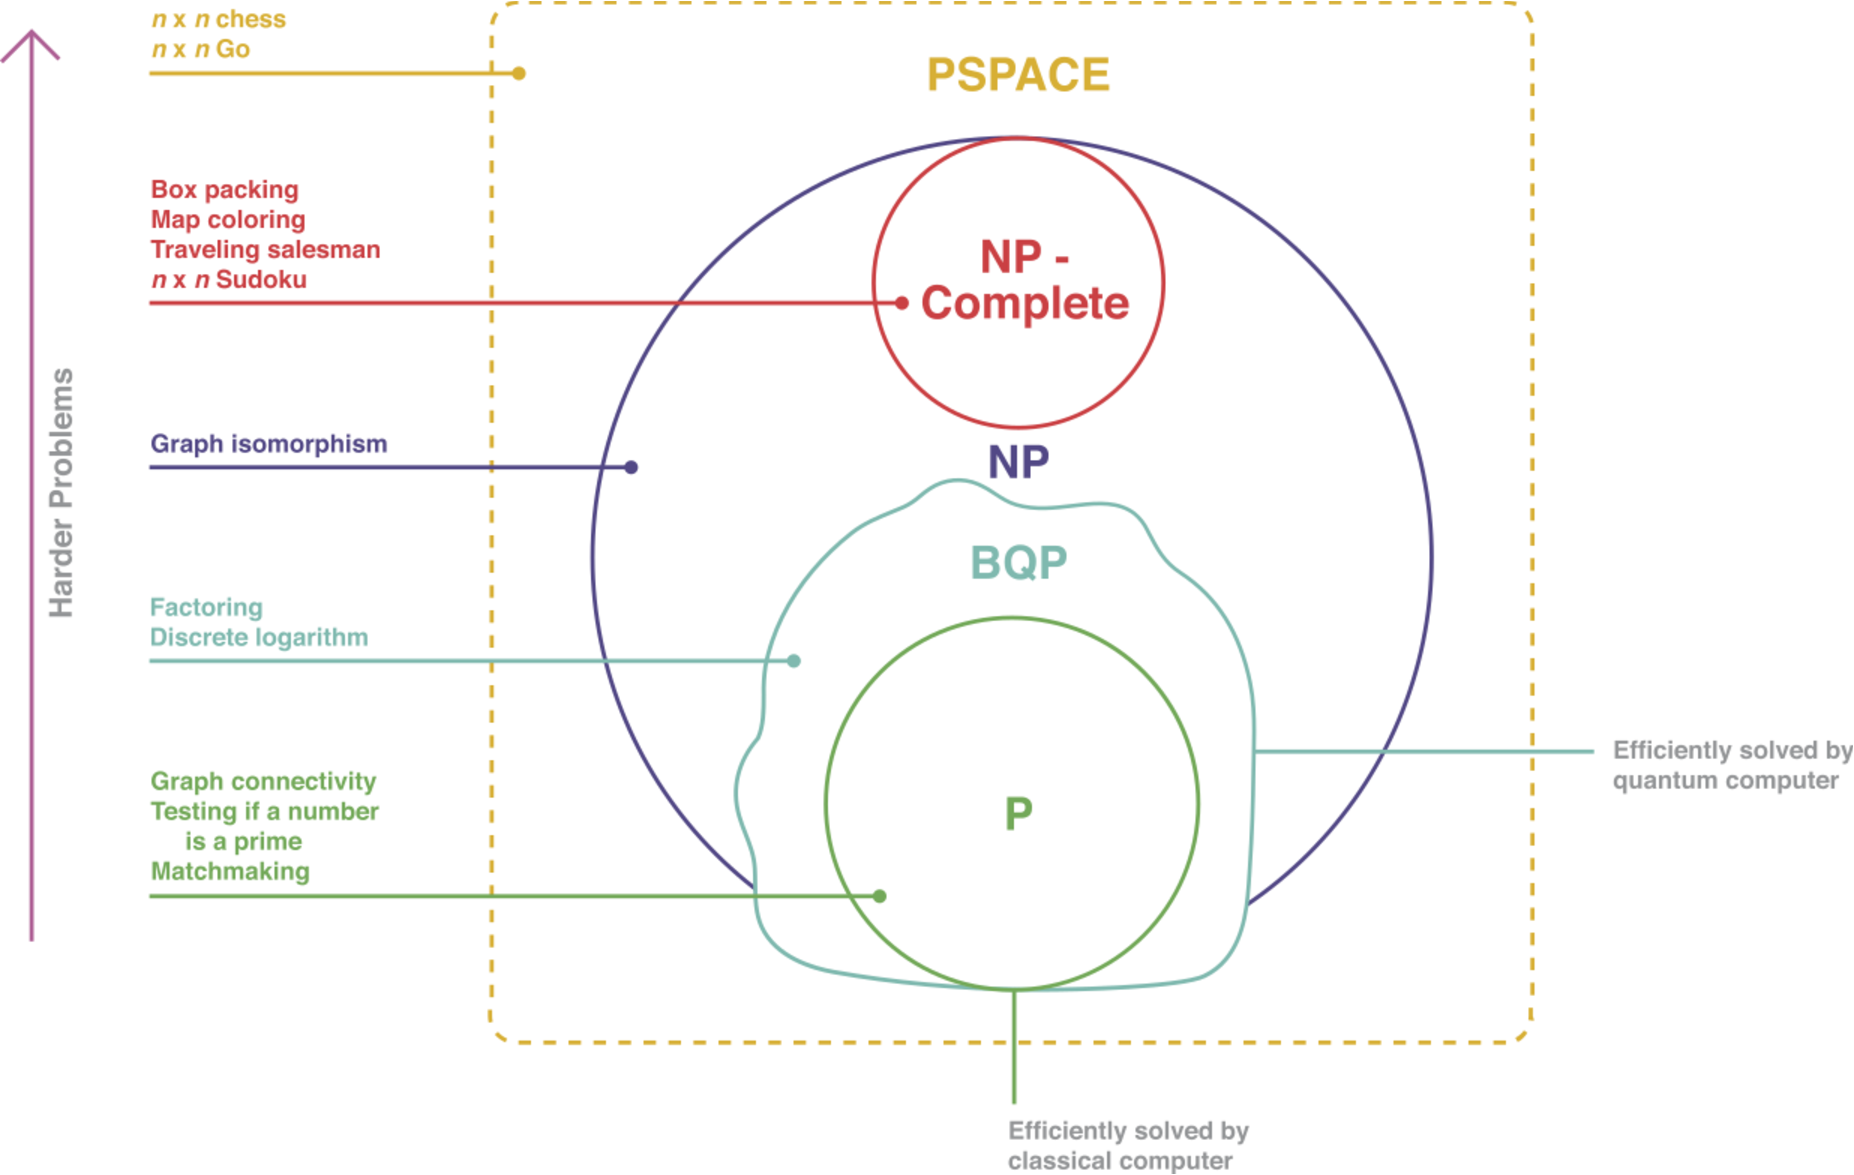
\includegraphics[width=.9\linewidth]{figures/complexity_hierarchy.pdf}
        \caption{A diagram illustrating the hierarchy of several important complexity classes. The exact relation between $\NP$ and $\BQP$ is not yet known. Image by MIT OpenCourseWare.}
    \end{figure}

    \section{Quantum Computing for Scientific Problems} \label{sec:quantum-science}
    While we are still in the very early stage of quantum hardware development, theorists have been finding applications in a variation of (scientific) fields.
    As of writing this, we are currently in the noisy intermediate-scale quantum (NISQ) era of quantum hardware~\cite{preskill2018quantum}.
    These current quantum computers have about 50-100 noisy qubits.
    Due to noise, errors may occur in these quantum systems and greatly limit their ability to do useful computations.
    On this scale there are limited applications for these machines (such as exploring many-body quantum physics), and it will take more and better qubits to really change the world.
    When we discuss applications of quantum computers, we assume access to a fully universal fault-tolerant quantum computer\footnote{Fault-tolerant quantum computers are quantum computers capable of handling any errors~\cite{oud2019introduction}. This is necessary to carry out meaningful computations.}, unless noted otherwise.
    
    \subsection{Quantum Chemistry}
    Quantum chemistry is probably the most promising application for quantum computing, both for NISQ and fault-tolerant quantum computers.
    Since the founding of the field of quantum mechanics, we have been able to describe the state of a quantum-mechanical system by solving the Schr{\"o}dinger equation~\cite{griffiths2018introduction}.
    However, the complexity of a quantum system grows exponentially with the number of particles.
    As ~\textcite{dirac1929quantum} noted: \say{\emph{The exact application of these laws leads to equations much too complicated to be soluble.}}
    This makes classical computers unfit for simulating quantum systems efficiently.

    It is believed that quantum computers will have applications in chemistry, biology, drug discovery, and materials science~\cite{mcardle2018quantum}.
    Several quantum algorithms have been proposed to solve problems in chemistry more efficiently~\cite{lidar1999calculating, kassal2008polynomial, aspuru2005simulated, vqe}.
    However, currently available NISQ hardware restricts these experiments to focus only on small molecules that we can already simulate classically.
    
    A fundamental problem in computational chemistry is finding the ground-state energy level of molecules~\cite{aspuru2005simulated}.
    This has also been a main area of research in the field of quantum computational chemistry.
    There are two well-known quantum algorithms for finding the ground-state of a molecule.
    The quantum phase estimation algorithm (QPE) is one that offers an exponential speedup over classical algorithms.
    However, it requires a quantum computer to stay coherent for millions to billions of quantum operations, compared to the tens to hundreds achievable in the near-term.
    An alternative algorithm suited for NISQ devices named the variational quantum eigensolver (VQE) was recently proposed~\cite{vqe}.
    It greatly reduces the quantum resources required by using classical optimization methods combined with a short quantum subroutine for measuring the expectation value of a Hamiltonian.
    The QPE and VQE algorithms can more generally be described as finding eigenvalues of a unitary operator.
    This has use cases outside chemistry such as determining the results of internet search engines~\cite{page1999pagerank}, and designing new materials and drugs~\cite{golub2000eigenvalue}.
    
    \section{Conclusion} \label{sec:conclusion}
    
    \printbibliography
\end{document}